\documentclass{article}
\usepackage[utf8]{inputenc}

\title{ECON 5253 PS1}
\author{Benjamin Fillmore}
\date{January 29 2021}

\usepackage{natbib}
\usepackage{graphicx}

\begin{document}

\maketitle

\section{Introduction}
This is the introduction, hello everybody. I left the graphic of the universe because I felt it added some fun - jazzed it up a bit.

\begin{figure}[h!]
\centering
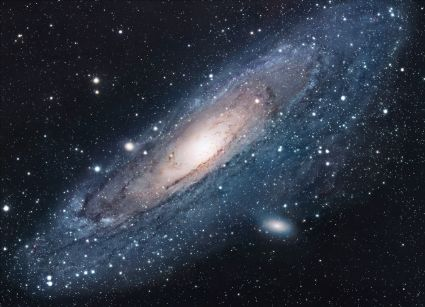
\includegraphics[scale=1.7]{universe}
\caption{The Universe}
\label{fig:universe}
\end{figure}

\section{Body}
I'd say I got into Economics as a major because the theoretical approach to our daily lives seemed really interesting. That has pretty consistently morphed as I take more classes and focus on different components within the field. When I joined the BA/MA program here I got really excited just how powerful the tools at our disposal were. I took this course specifically because learning more about Data Science rather than Data Analysis seemed really interesting. Further, coding is something I think I can't ever know enough about; I essentially always want to be learning more. I also really enjoyed Econometrics last semester and wanted to expand on that. I would like to potentially create a predictive model for rider types within cycling, based around power curve, Height:Weight, Heart Rate, and as much data as I can possibly gather. It would be interesting to see whether or not one's specialty within the sport of cycling could be predicted effectively based on these variables. Throughout this course I'd like to build my R abilities, but I'm more excited at the possibility of establishing myself in Python, SQL, and Julia. I see in the job market I'm lacking crucial skills in using Hadoop/Spark, SQL, and more advanced algorithm building in Python. I'd really like to move to Austin and work in Data Science and Business Analysis. 

\section{Conclusion}
Hope that clears up some aspects of my motivations and satisfies all required of me for this assignment.

\section{Equation}

\begin{equation}
a^2 + b^2 = c^2
\end{equation}


\end{document}
